A browser interface that allows the user to interact with the entire system.

\begin{figure}[h!]
	\centering
 	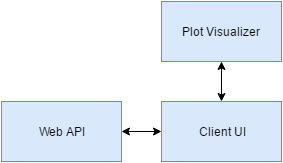
\includegraphics[width=0.60\textwidth]{images/web_client_layer}
 \caption{Example subsystem description diagram}
\end{figure}

\subsection{Web API}
The Web API makes calls to the web service layer. It also stores and provides user authentication credentials.

\subsubsection{Assumptions}
The Web API cannot assume the web service layer is always operating and will respond.

\subsubsection{Responsibilities}
It should maintain connection to web service layer. It should pass all requests from other subsystems. It should keep user authentication credentials so that API calls can be validated.

\subsubsection{Subsystem Interfaces}

\begin {table}[H]
\caption {Subsystem interfaces} 
\begin{center}
    \begin{tabular}{ | p{1cm} | p{6cm} | p{3cm} | p{3cm} |}
    \hline
    ID & Description & Inputs & Outputs \\ \hline
    \#01 & HTML Interface & \pbox{3cm}{HTML Requests} & \pbox{3cm}{JSON Objects}  \\ \hline
    \end{tabular}
\end{center}
\end{table}

\subsection{Plot Visualizer}
Take data and convert it into image. It should take the plot data and graph out the elements and generate a visual example.

\subsubsection{Assumptions}
The input data is valid.

\subsubsection{Responsibilities}
It should convert data to image and be able to generate visual example.

\subsubsection{Subsystem Interfaces}
\begin {table}[H]
\caption {Subsystem interfaces} 
\begin{center}
    \begin{tabular}{ | p{1cm} | p{6cm} | p{3cm} | p{3cm} |}
    \hline
    ID & Description & Inputs & Outputs \\ \hline
    \#01 & Plot data & \pbox{3cm}{JSON Object} & \pbox{3cm}{Image or JS Canvas}  \\ \hline
    \end{tabular}
\end{center}
\end{table}

\subsection{Client UI}
A JavaScript based UI to allow the user to see the status of the farmbot, send commands, and schedule various activities.

\subsubsection{Assumptions}
The client browser will run the needed JavaScript. Unsupported browsers will be notified and rejected.

\subsubsection{Responsibilities}
The Client UI should maintain minimal resource usage to maintain the expected functionality.

\subsubsection{Subsystem Interfaces}
\begin {table}[H]
\caption {Subsystem interfaces} 
\begin{center}
    \begin{tabular}{ | p{1cm} | p{6cm} | p{3cm} | p{3cm} |}
    \hline
    ID & Description & Inputs & Outputs \\ \hline
    \#01 & Javascript & \pbox{3cm}{User Interaction} & \pbox{3cm}{Web Page}  \\ \hline
    \end{tabular}
\end{center}
\end{table}